\chapter{\Edgeworth: diagrammatic problem authoring at scale}
\label{chp:edgeworth}

\begin{figure}[h]
    \centering
    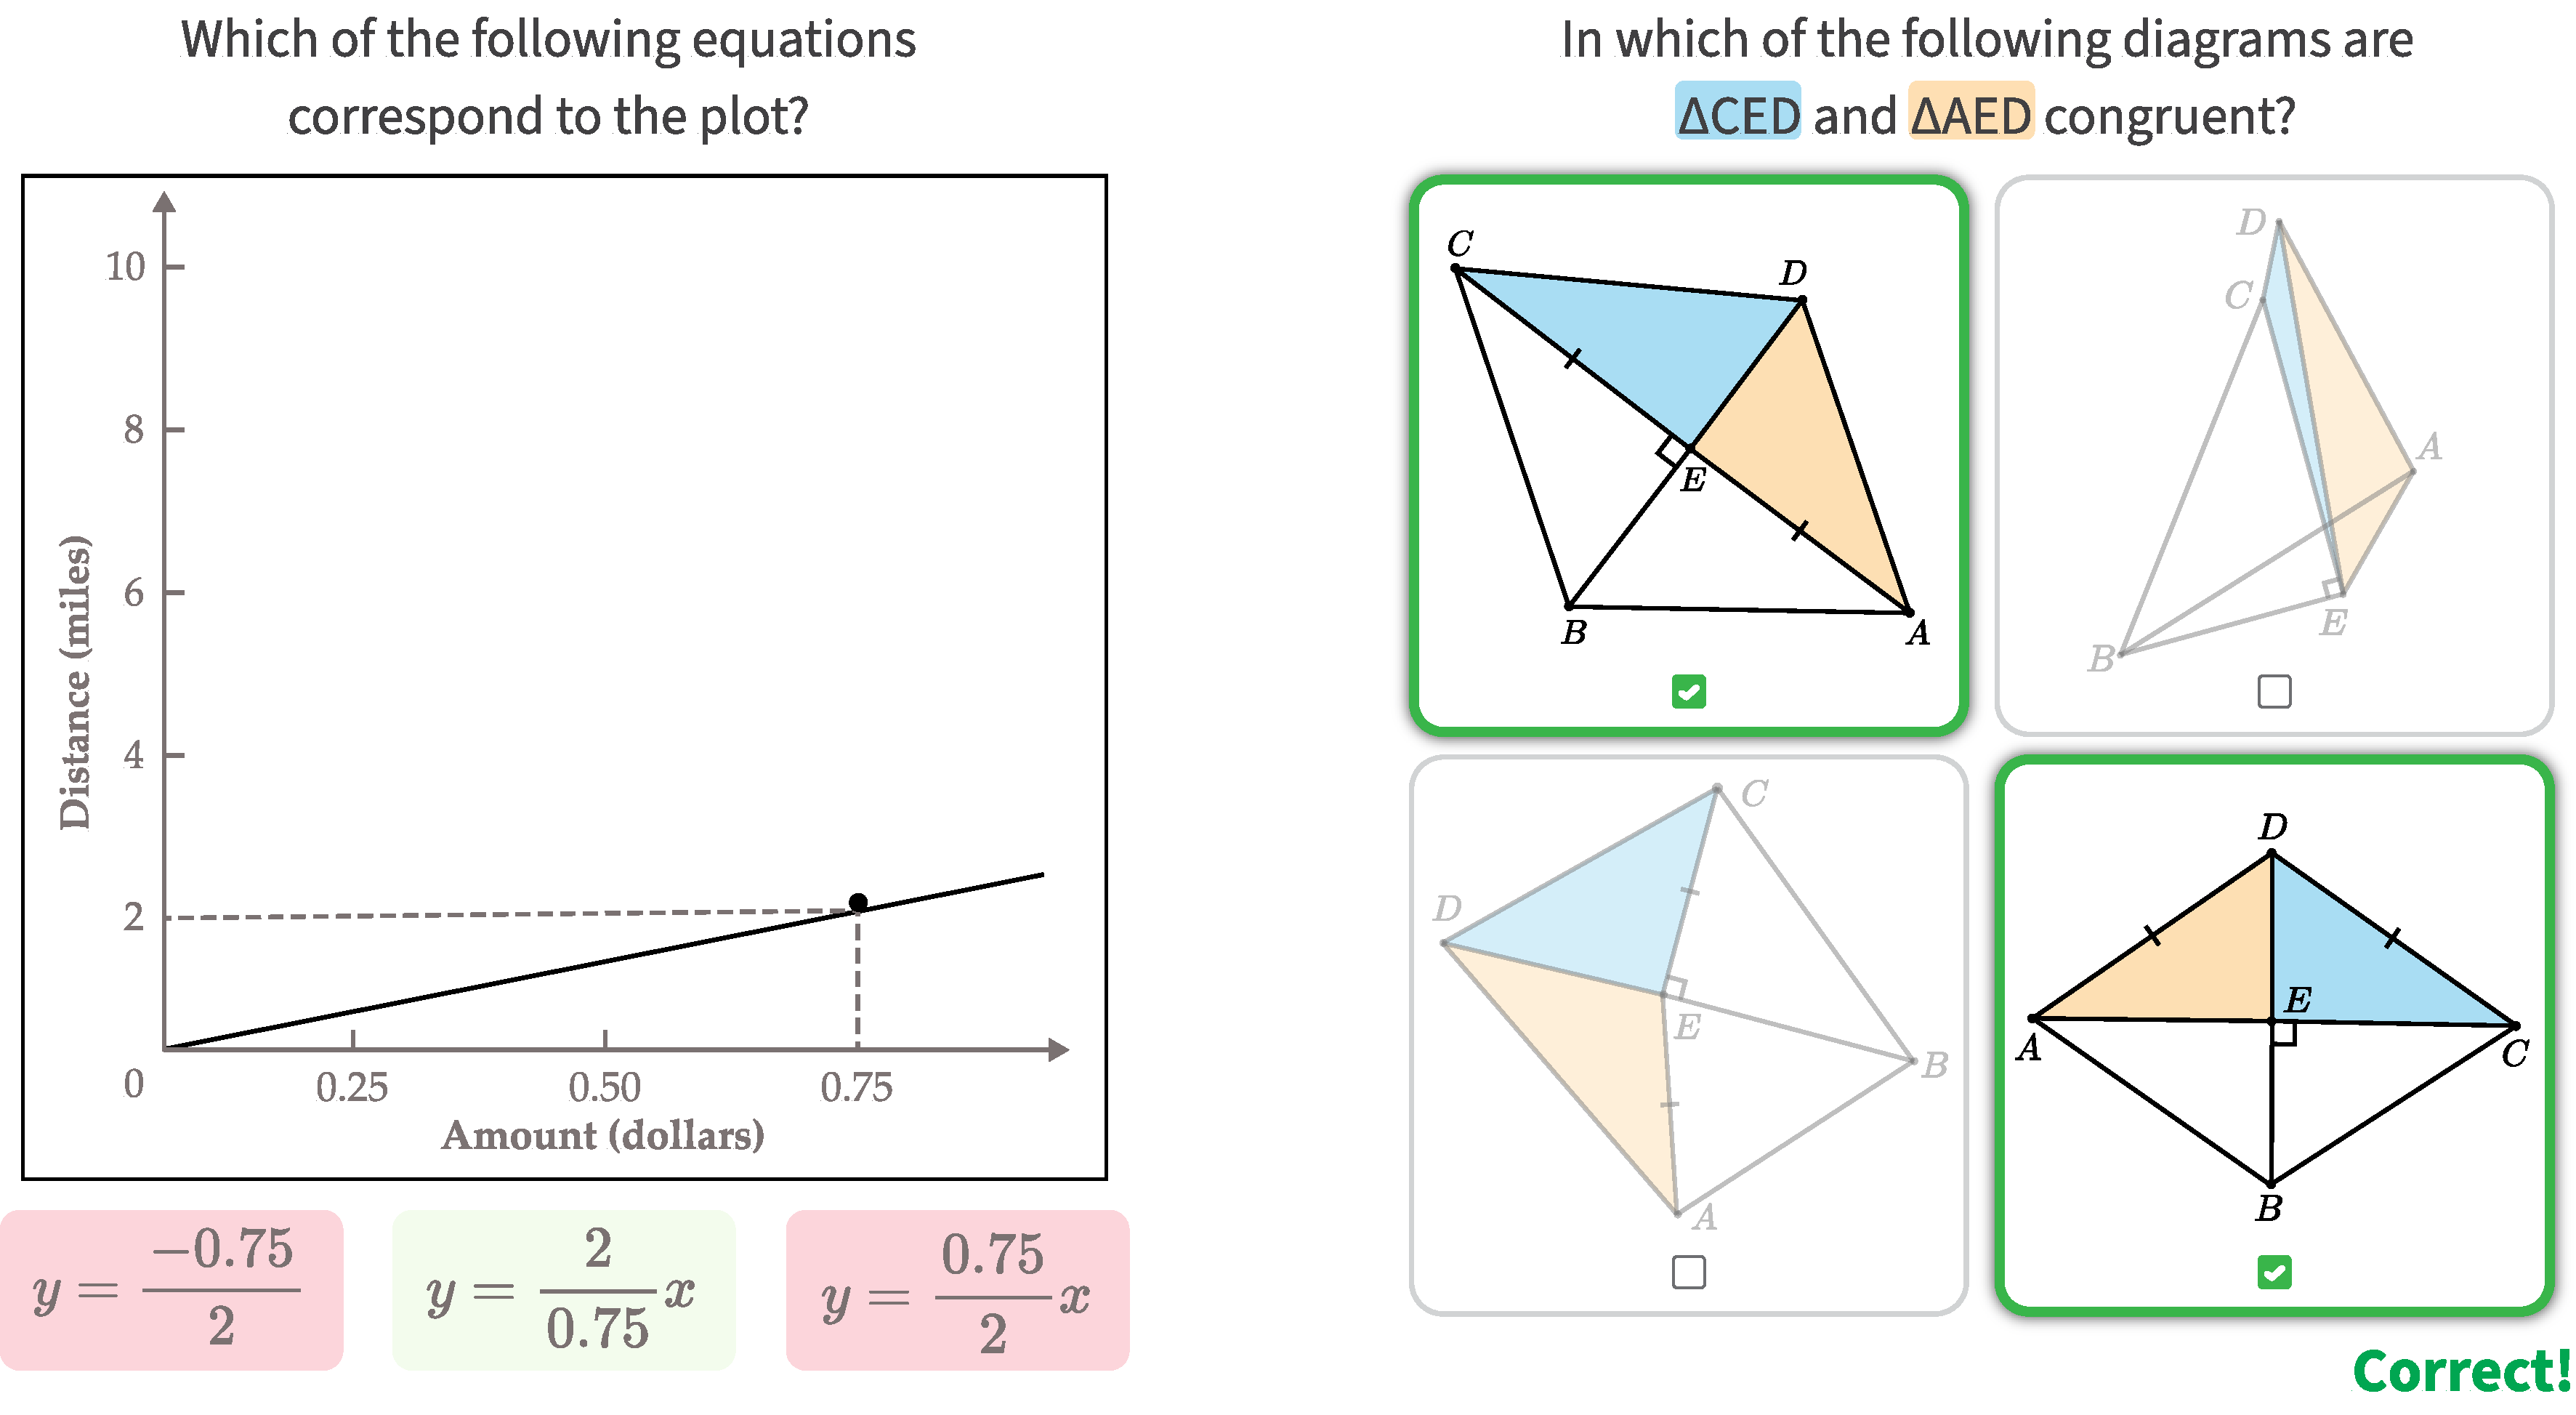
\includegraphics[width=0.45\linewidth]{assets/chapter-3/translation-problem.pdf}
    \hspace{5pt}
    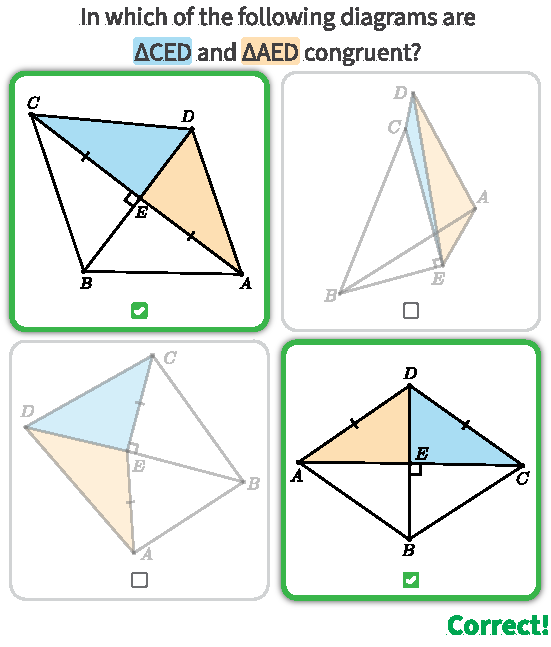
\includegraphics[width=0.45\linewidth]{assets/chapter-3/edgeworth-problem.pdf}
    \caption{\textbf{left}: a translation problem that helps students discern the structure of linear equations (adapted from~\cite{perceptualLearning}). \textbf{right}: an \Edgeworth generated problem that trains student to recognize diagram configurations~\cite{Koedinger1990a} for triangle congruence.}
    \label{fig:translation-problem}
\end{figure}

\vspace{10pt}

Effective use of visual representations requires a certain level of \emph{representational fluency} that's achievable through deliberate practice and repetition~\cite{metarepresentation, representationalFluency}. Recognizing how words, symbols, and diagrams relate to each other is an important first step of achieving fluency. Prior work has shown that these contrasting cases, \ie, discrimination and mapping, among representations significantly improve students' ability to translate among representations~\cite{perceptualLearning}.

To train students' representational fluency, educators often create problem sets that involve numerous contrasting cases of a particular visual representation. For instance, \cref{fig:translation-problem}~shows two examples of \emph{translation problems}, where the problem asks students to determine diagrammatic \emph{instances} and \emph{noninstances} of a textual description and vice versa. Importantly, these instances and noninstances have varying degrees of differences from the given diagram or text, and carefully picking examples on this spectrum has a big impact on learning~\cite{samenessAndDifference}.

Unfortunately, authoring diagrammatic problems remains a tedious, manual process. Our formative interviews show that educators have difficulties creating simple shapes using existing tools. Limited by the tools, educators don't have support to create enough problems and resort to copy-pasting and manual editing. They expressed desires for tools that understand the diagrams and allow them to make semantically-consistent tweaks to diagrams.

In this chapter, I discuss \Edgeworth, a tool that supports an automated and scalable diagrammatic problem authoring workflow. 

\section{Formative interviews}
\label{sec:edgeworth-formative}

To inform the design of \Edgeworth, I conducted semi-structured interviews of teachers, textbook authors, and learning engineers that have experience creating instructional material, authoring problems, or developing e-learning tools that include mathematical diagrams. The interview questions ask about what roles visuals play in the educational material, how they are connected to surrounding content, and how students interact with visual content. This formative study aims to understand the gaps between affordances of current tools and ideal workflows of content creators, and the need for automation and mass production of visual content. Participants are asked to share content they have created and discuss the creation process in detail.

\subsection{Need for diagrammatic contents}

Traditional educational materials, especially in higher education, tend to emphasize \quotei{procedures, memorization, and symbolic manipulation} (P6). As a result, students often become \quotei{symbolically good} and do not develop \quotei{good conceptual understanding} (P3). Visual content like diagrams and graphs provide alternative representations that help students \quotei{develop intuition and become better problem solvers} (P3). As a result, most of our participants include visuals in their instructional materials such as problem sets and lecture notes. Some also ask students to draw, annotate, and explain diagrams (P1, 2, 6). 

\subsection{Visual content in instruction}

P2 would deliberately encourage students to learn \quotei{multiple representations} and made diagrams central to their math and programming curricula. For instance, a typical problem set in a pre-calculus class will have either problems with diagrams, or students have to \quotei{produce a drawing if no pictures are given.} To improve students' \quotei{visual fluency,} P1 incorporates visualization tools such as GeoGebra in their middle school math classroom. Students draw in in-class activities and homework assignments. P1 found that students \quotei{benefit from using a diagram,} but also refer to the \quotei{curse of knowledge} when teaching students how to use diagrams: students need deliberate practice to use visuals successfully, but existing instruction tends to under-train them. When students practice with visuals, instructors like P6 also gain richer feedback of students' level of understanding: \quotei{when the students drew diagrams to figure out the answer. I actually learned more from this than 10 similar problems without the picture.}

\subsection{Need for better tools}

Many aspects of content authoring can be repetitive and iterative. Authors typically create \quotei{multiple similar examples} (P1) and \quotei{variants of classroom examples in problem sets} (P6). In addition, they iterate on their content often, even \quotei{re-do my courses every semester} (P2) in some cases. Participants face a trade-off when authoring visual content: visuals are much harder and time-consuming to create, especially when variations and frequent changes are required in instructional materials, which is often the case. When authoring practice problems, P1 struggles to \quotei{create simple shapes by myself} and always ends up \quotei{copy-pasting and searching online} repeatedly. As a result, P1 tends to \quotei{reuse [a few of my existing diagrams. Thinking about having to do it all over again for another class is just too much.} To make visual content authoring time efficient, P2 and P5 developed a custom pipeline for authoring problem sets and quizzes using programming tools. Similar to problems described in~\cite{naturalDiagramming}, these tools often lack support for \quotei{high-level tweaking of my diagrams} (P2) and \quotei{are a pain to use because the language is not semantic and hard to use for non-programmers.} (P5) 

\section{Mutation-based diagram generation}
\label{sec:mutation}

Educators simply don't have enough time to produce good-looking diagrams, not to mention the amount and variety of diagrams required for training students to be fluent in visual representations. Therefore, a key pain point to automate is diagram generation. Importantly, the generated diagrams have to be meaningful and need to include contrasting cases of the same subject matter. 

In \Edgeworth, I propose to \textbf{generate a large pool of diagrams by mutating the \Substance program in a \Penrose trio}. Compared with general-purpose programming languages, \Penrose DSLs have unique advantages: \Domain is a meta-language that precisely defines the available program constructs in \Substance, which helps define the mutation search space. Moreover, it’s easier to make sense of mutation on \Substance, because it corresponds to the domain-specific vocabulary of diagram authors. 

At a high level, the \Edgeworth mutator takes in a \Penrose trio and a small configuration file, and simply generates an arbitrary number of \Substance programs. Constrained by the configuration, \Edgeworth mutates the \Substance program (\emph{prompt program}) by applying a series of program mutations to get a \emph{mutant} \Substance program. For each mutant, the system then uses the original \Style and \Domain programs to render a diagram. 
 
\begin{figure}[h]
    \centering
    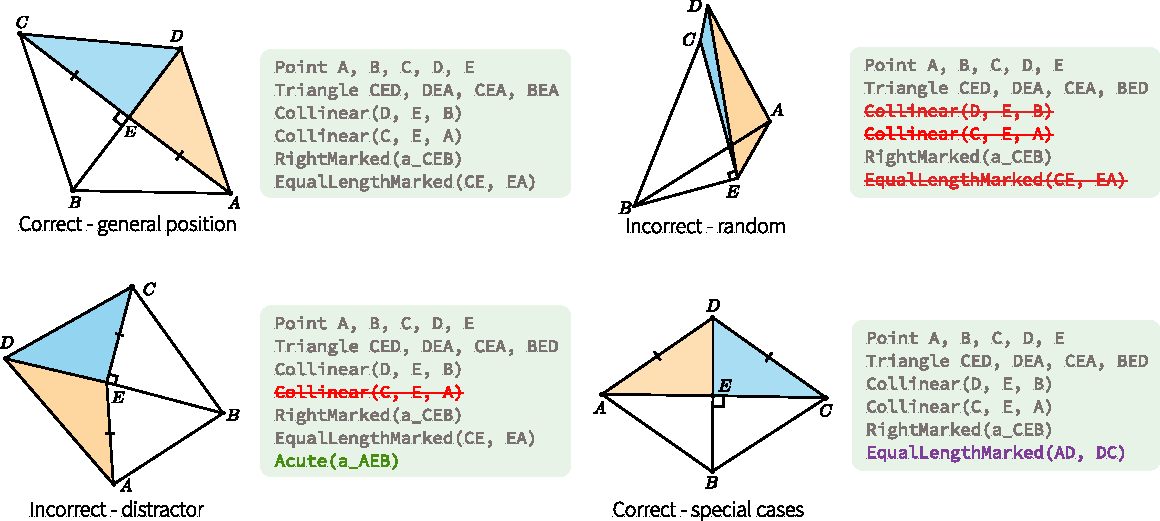
\includegraphics[width=\linewidth]{assets/chapter-3/answer-types.pdf}
    \caption{Four example classes of mutants generated by \Edgeworth. \textbf{Top-left}: the original prompt program, representing a general correct instance. \textbf{Bottom-Left}: an incorrect noninstance that only slightly differs from the original prompt semantically. \textbf{Top-right}: an incorrect noninstance that differs significantly from the prompt. \textbf{Bottom-right}: a correct instance that's a corner-case of the prompt.}
    \label{fig:answer-types}
\end{figure}

Since \Substance is a small declarative language, \Edgeworth uses a set of pre-defined, high-level mutation operations listed below. 

\begin{itemize}
    \item \textbf{Add} Appends a statement to the \Substance program.
    \item \textbf{Delete} Removes a random statement from the \Substance program.
    \item \textbf{Cascading Delete} Removes a random statement and all other references to that statement.
    \item \textbf{Swap Arguments} Reorders the arguments passed into a statement. \eg, if \sub{A} and \sub{B} are \sub{Triangles}:
    
            \sub{Similar(A, B)} $\rightarrow$ \sub{Similar(B, A)}
    \item \textbf{Swap-In Arguments} Replaces the arguments passed into a statement with other arguments defined in scope. \eg, if \sub{A, B, C, D} are \sub{Points}:
            
            \sub{s := MkSegment(A, B)} 	$\rightarrow$ \sub{s := MkSegment(C, D)}
    \item \textbf{Replace Statement Name} Replaces a statement with a different statement that takes the same type of arguments and has the same return type. \eg, given that \sub{T} is a \sub{Triangle}:
            
            \sub{Right(T)} $\rightarrow$ \sub{Obtuse(T)}
    \item \textbf{Type Change} Replaces a statement with a new one that takes the same number and type of arguments, but does not necessarily return a value of the same type. \eg, if \sub{E} is an \sub{Angle}:
            
            \sub{Segment s := Bisector(E)} $\rightarrow$ \sub{Right(E)}
\end{itemize}

These mutations are all done safely at the level of the abstract syntax tree (AST) and \Edgeworth maintains a local context and symbol table, so operations will not introduce errors. The configuration file contains a set of rules to filter down the search space by statement types and specify the kinds of mutations allowed. 

Authoring contrasting cases require different classes of diagrams: those that correctly correspond to the textual/symbolic description and others that don't. Importantly, nearest neighbors of the prompt program seem to have great education values, \ie, ``near misses'' and ``near hits.'' Knowing the correctness of a mutant also helps with automated grading of problems. 

Although \Edgeworth generates syntactically valid mutants, the system doesn't know whether a mutant is semantically consistent with the prompt \apriori. Currently, the system uses the graphical constraints to determine semantic consistency. Specifically, it uses an energy-based heuristic by performing \textbf{cross-instance energy evaluation (CIEE)} of each mutant. Suppose \Edgeworth mutates the prompt program $P$ to mutant $P'$ and generates a diagram $D'$ from $P'$. the system can compute the cross-instance energy of $D'$ by 1) checking if all of the constraints generated from $P$ are met by $D'$ and 2) run the objective function defined by $P$ on $D'$ and check if the $D'$ is at a local minimum.  In other words, the \Penrose optimizer determines if the diagram $D'$ generated from mutated program $P'$ is a good fit for the prompt program.

\vspace{10pt}

\begin{figure}[h]
    \centering
    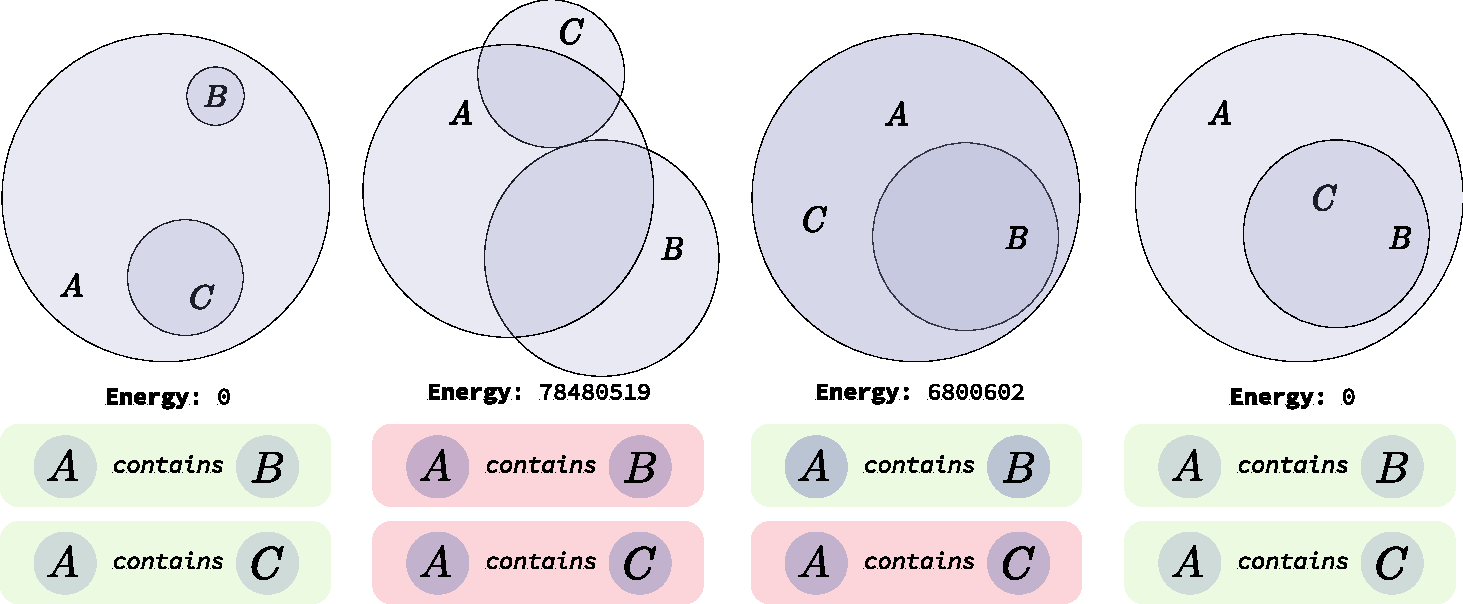
\includegraphics[width=\linewidth]{assets/chapter-3/ciee.pdf}
    \caption{An example of CIEE, where the leftmost is the prompt program $P$ and its corresponding diagram $D$. The overall energy value is $0$. The right three are instances of $P'$, on which the constraints from the prompt are evaluated. The middle two are \textit{semantically inconsistent} with the prompt and have high energy values. The rightmost is \textit{semantically consistent} with the prompt and therefore has an energy value of $0$.}
    \label{fig:ciee}
\end{figure}

\vspace{10pt}

\begin{proposed}
\textbf{CIEE robustness.} CIEE showed some promise on a limited set of examples, but further evaluation is needed to see the robustness of this heuristic. For instance, how much does this method depend on the qualities of the \Style program that defined the constraints? If the mutant significantly differs from the prompt (\eg, missing most identifiers from the prompt), is this heuristic still useful?

\textbf{\Domain language extensions.} None of the predefined mutations listed above carry any mathematical semantics because \Domain doesn't contain enough information. For instance, many mathematical predicates have reflexive, symmetric, transitive, and substitution properties, but \Domain only encodes basic type definitions. For a more precise notion of correctness, I plan to extend \Domain to model such properties, and use them in the \Edgeworth mutator, possibly together with CIEE, to generate higher quality mutants.  

\end{proposed}

\section{Preliminary evaluation of the \Edgeworth mutator}
\label{sec:edgeworth-prelim-eval}

In preliminary work, we evaluated the system by recreating problems in a middle-school geometry textbook \cite{holtGeometry}. We examined all 53 diagrammatic problems in the chapter review sections and picked a representative subset of 24 problems and implemented them in \Edgeworth. For each textbook problem, the prompt is reframed so that the diagram accompanying the original problem can be considered a correct answer. Then, we consider possible answers to the posed question, including ``distractors''---answers that are designed to tempt students with limited conceptual understanding---as well as correct ``special cases''. We then describe the original diagram as a prompt \Substance program and pass it to \Edgeworth, which generates numerous answers to the original problem.

We examined sets of 20 diagrams generated by \Edgeworth based on various prompt programs. Each program was mutated 1-3 times and the correctness of each diagram was determined manually. We found that while \Edgeworth easily generates a variety of correct and incorrect diagrams, careful selection of configuration parameters was often required to get more ``interesting'' diagrams (correct special cases, distractors).

\begin{proposed}
\label{prop:config-usability}
\textbf{Usability of the \Edgeworth configuration.} As noted above, results from the \Edgeworth mutator are sensitive to the configuration. For instance, a statement in the \Substance program might be particularly more suitable for mutations than others (perhaps because it contributes to the correctness of the problem.) Under- or over-specifying mutations in the configuration might lead to a pool of ``noisy'' diagrams. I propose to conduct a light-weight case study with a handful of problems to identify the key to successful configurations. With that insight, we can either improve the configuration format or explore other modes of interaction.
\end{proposed}

\section{Mutation paths as problem templates}
\label{sec:mutation-paths}

\begin{proposed}
After generating a pool of diagrams, the author then picks a subset of them for a single \emph{problem instance}. For each generated diagram, \Edgeworth keeps a record of the series of mutations performed on the prompt program (\emph{mutation path}) to the mutant. For a multiple choice problem with four options, there will be four mutation paths from the prompt. Together these paths form a \emph{problem template}.

A problem template is specific to a prompt, so it's unlikely to be reusable for generating other problem instances. However, many problems might share the same instructional goal such as teaching students the conditions for the Hypotenuse-Leg (HL) theorem. While the choice of names and diagram design may differ, the core structure is the same: two instances of congruent triangles satisfying HL and two noninstances of non-congruent triangles. Encoding this information can further scale up problem authoring. 

I propose to \textbf{investigate common structures among problem templates and encode them as problem template specifications that are generalizable to multiple prompts}. 

\end{proposed}

\section{By-example workflow for authoring at scale}
\label{sec:edgeworth-by-example}

With the \Edgeworth mutator, the primary mode of interaction is picking examples from the mutant pool and editing the configuration to narrow down the search space. In some cases (see \cref{prop:config-usability}), the author might want to write a few examples from scratch, or prefer to manually make slight tweaks to examples in the mutant pool. I propose to \textbf{create a programming-by-example workflow, where the author manually creates a few diagrams and \Edgeworth generates a bigger pool of diagrams with similar properties}.

\vspace{10pt}
\begin{figure}[h]
    \centering
    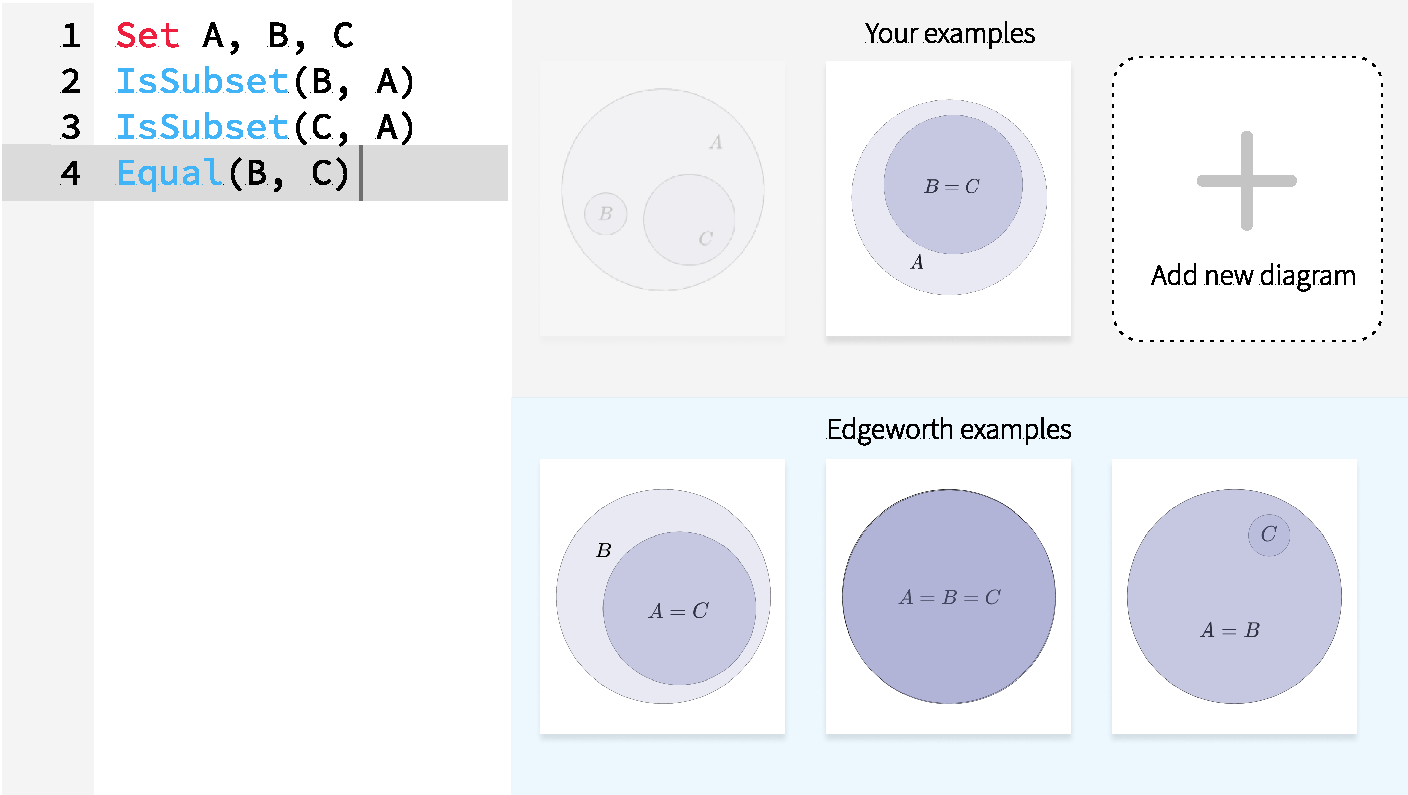
\includegraphics[width=\linewidth]{assets/chapter-3/synthesis-driven-workflow.pdf}
    \caption{User interface mock-up of a by-example workflow in \Edgeworth.}
    \label{fig:synthesis-driven-workflow}
\end{figure}
\vspace{10pt}

For example, if \Edgeworth fails to generate a pool of useful diagrams, the author can manually create a few examples by directly editing the prompt program. In \cref{fig:synthesis-driven-workflow}, the author adds the \sub{Equal(B, C)} predicate. Their intent is to include the edge case of proper subsets in this problem, where some of the subset relations are actually equality. \Edgeworth generates a set of similar examples that add \sub{Equal} predicates with existing identifiers in different ways. 

The addition of \sub{Equal(B, C)} is effectively a user-generated mutation, and \Edgeworth needs to understand this mutation to generate similar instances. Currently, the \Edgeworth synthesizer matches a series of author edits to predefined mutations. Once the synthesizer finds a path, it can then inform the mutator to generate examples with similar properties (\ie, including the edge case of equal sets). 

\begin{proposed}
\textbf{Generalized mutation paths} Similar to templates, the by-example workflow also requires a generalizable encoding of mutations. I plan to experiment with a few possible formats such as (1) another mutator configuration and (2) mutation paths with ``holes.''
\end{proposed}

\section{Evaluation}

\begin{proposed}
\textbf{Usability study of \Edgeworth.} I propose to evaluate the usability of \Edgeworth by recruiting authors to perform content authoring tasks with the \Edgeworth prototype. For example, the participants may be asked to author a problem set of 10 diagrammatic problems. The goal of this study will be to identify missing features, usability problems, and opportunities for simplification. The study may include several rounds with increasingly high-fidelity prototypes. After each round, I will refine the design and implement the next prototype. Here are some possible research questions:
\begin{itemize}
    \item  What are the key design considerations for diagrammatic problem authoring? How do they fit with the features of \Edgeworth?
    \item How do authors prefer to work with \Edgeworth? When do they opt to write a configuration file and generate many diagrams? When do they use the by-example workflow? Do they mix the two workflows?
    \item How does the experience compare to their existing tools? How can \Edgeworth incorporate useful parts of them? 
\end{itemize}
\end{proposed}

\section{Related work}
\label{sec:edgeworth-related}

\subsection{Using contrasting cases to improve representational fluency}

Representational fluency refers to the ability to quickly understand a visual representation and to use it to solve domain-specific tasks~\cite{multipleReps}. To become representationally fluent, an important first step is to identify meaningful aspects of a particular representation. \citet{perceptualLearning} show that mapping between symbolic and visual representations leads to intuitions about the way equivalent structures relate to each other. The learning that results from constructing connections between symbols and diagrams can be more flexible. Students are better at transferring their learning from the problems they have explicitly practiced to more open-ended problems and their conceptual understanding is better~\cite{25learning}. 

In addition to mapping between representations, \citet{samenessAndDifference} also showed that contrasting cases help students discern crucial parts of a particular representation. Early on, students benefit from discerning instances and noninstances that differ in only one dimension of variation. As students become more fluent, a \emph{fusion} of multiple varying dimensions in problems may be necessary~\cite{fusion}.

\subsection{Multiplicity of examples and problem generation}

In addition to training representational fluency, multiple examples and repeated, varied practice are well-documented strategies for broader learning goals in the learning science literature. Many studies have demonstrated substantial STEM learning benefits for multiple worked examples per topic \cite{PBB07}. Equally important is research indicating the importance of active learning \cite{CW14, DMM19} and repeated practice \cite{deliberatePractice, SSL98} that occurs within varied contexts \cite{PV94, RT07} and involves direct explanatory feedback \cite{perceptualLearning}.

As a result, a number of authoring tools exist for large-scale production of examples and practice problems. Intelligent Tutoring Systems (ITS) are automated curricula that often include worked examples and practice problems that are customized to individual students. The Cognitive Tutor Authoring Tools (CTAT) is an ITS authoring platform~\cite{CTAT}. CTAT has a ``Mass Production'' feature that lets the user create a problem template and insert problem-specific values via a spreadsheet~\cite{massProduction}. The ASSISTment builder allows authors to ``variablize” numerical values in problem templates for automatic generation~\cite{ASSISTment}. In the computer-aided education literature, a number of systems were also proposed for problem generation~\cite{compEduCACM, synthDeduction, synthGeometry} In both lines of work, most systems don’t tackle the problem of diagram generation—they mostly generate symbolic problems and examples. Notably, \citet{synthGeometry} generated ruler-and-compass geometry constructions automatically, which is a significantly narrower domain than what \Edgeworth targets. 
